\chapter{Trabalhos Relacionados} % (fold)
\label{cha:trabalhos_relacionados}

Ao considerar que o presente trabalho demonstra uma metodologia para a coordenação de uma equipe de agentes robóticos para o transporte de objetos, será apresentado neste capítulo uma coleção de trabalhos que expõem técnicas e estratégias que tratam de problemas similares, e que serviram de inspiração para o procedimento aqui explicitado.

O capítulo está divido em duas sessões, as quais mais representam as sub-tarefas tratadas neste trabalho, são elas: (i) técnicas para a manipulação e transporte de objetos, (ii) mecanismos para controle e alocação de tarefas entre os agentes de uma equipe.

% -- considerando tanto métodos preênsil quanto não-preênsil

\section{Manipulação de Objetos} % (fold)
\label{sec:t_cnicas_de_manipula_o_de_objetos}

A manipulação de objetos é um tema de bastante interesse dentro do campo de pesquisa da robótica, ao considerar que existem maneiras diferentes de realizar a mesma, cada uma com características próprias, agregando à tarefas qualidades e graus de complexidade diferentes.
Como definido no Capítulo \ref{cha:introdu_o}, as técnicas relacionadas ao manejo de objetos serão dividas em duas categorias: (i) não-preênsil e (ii) preênsil.

\subsection{Manipulação Não-preênsil} % (fold)
\label{sub:manipula_o_n_o_pre_nsil}

As técnicas não-preênsil são aplicadas de forma geral em casos no qual o objeto a ser transportado é maior e/ou pesado, de modo que não possa ser erguido facilmente.
Possui uma vantagem em relação às técnicas preênsil, no fato do agente manipulador não necessitar de um contato contínuo com o item a ser transportado.

Para a realização do transporte utilizando uma das técnicas citadas a seguir, em sua maioria, o agente deve aplicar uma força sobre o objeto, principalmente utilizando seu próprio corpo, de modo a empurrar o mesmo em uma determinada direção, nomeadas como técnicas de \emph{PUSH}.

Tais técnicas foram desenvolvidas para a resolução do chamado problema \emph{box-pushing} definido por \cite{Mataric1995}, descrito como: dado um ambiente formado por itens poligonais rígidos, encontrar um caminho contínuo livre de obstáculos levando um objeto de uma configuração de origem para outra configuração desejada utilizando somente ações de \emph{PUSH} para mover o mesmo. Como demonstrado por \cite{Reif1979}, este é um problema \emph{PSACE-hard}, o que implica em ser \emph{NP-hard}.

O estado da arte no âmbito da manipulação não-preênsil compreende quatro tipos de táticas de movimentação dos objetos:
(i) \de{forcec} (\gl{forcec}) -- na qual os agentes impõem forças sobre o objeto de forma a segurá-lo fortemente, até que seja atingido um equilíbrio entre as mesmas,
(ii) \de{formc} (\gl{formc}) -- nesta técnica os agentes circundam o objeto sem a necessidade de aplicar forças sobre o mesmo,
(iii) \de{objc} (\gl{objc}) -- similarmente à \gl{formc}, os agentes são arranjados próximos ao objeto, de forma que o objeto fica sempre preso, e
(iv) \de{condc} (\gl{condc}) -- onde os agentes aplicam forças sobre o objeto somente em um determinado lado, condicionados pela necessidade do sistema (\cite{Eoh2011}). Estas técnicas estão ilustradas na Figura \ref{fig:non_preensile_methods}.

\begin{figure}[htpb]
  \centering
  \setlength{\fboxsep}{0pt}
  \begin{subfigure}[t]{0.45\textwidth}
    \centering
    \fbox{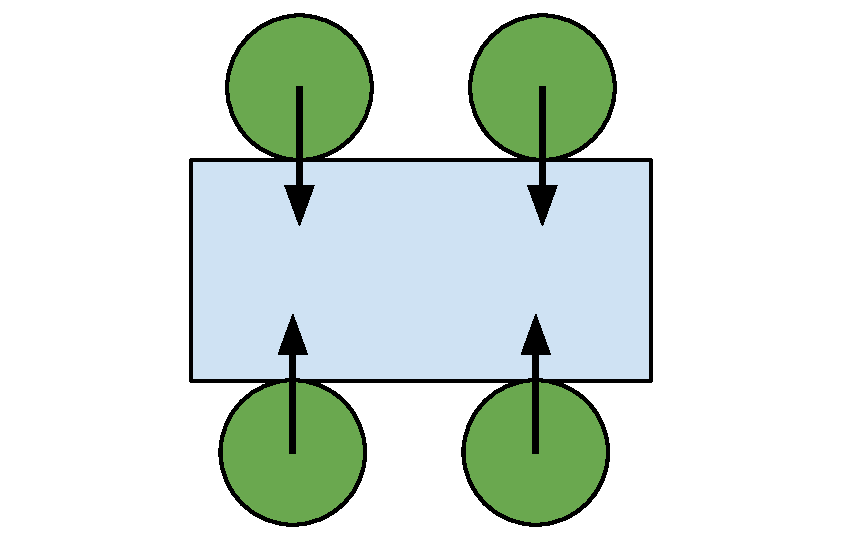
\includegraphics[width=0.9\textwidth]{img/libs/TransportTypeForceClosure.pdf}}
    \caption{\emph{Force Closure}}
  \end{subfigure}
  \hspace{0.2cm}
  \begin{subfigure}[t]{0.45\textwidth}
    \centering
    \fbox{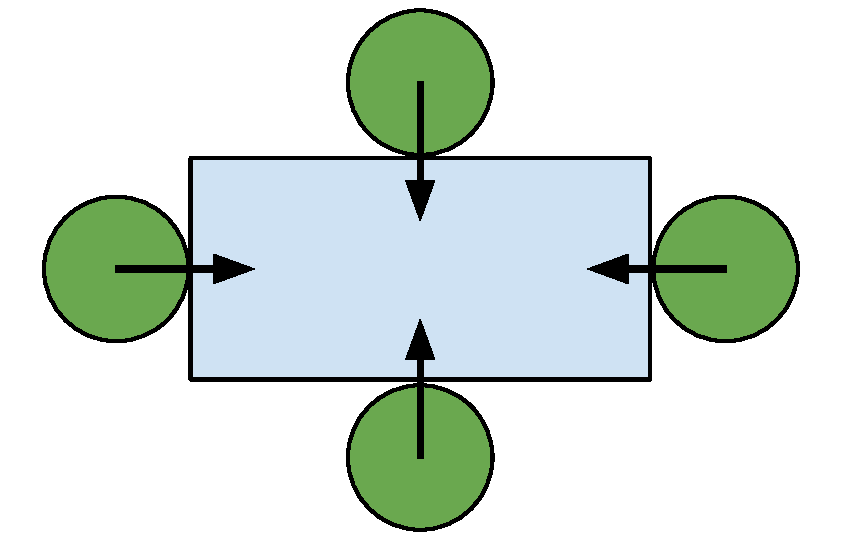
\includegraphics[width=0.9\textwidth]{img/libs/TransportTypeFormClosure.pdf}}
    \caption{\emph{Form Closure}}
  \end{subfigure}

  \vspace{0.3cm}
  \begin{subfigure}[t]{0.45\textwidth}
    \centering
    \fbox{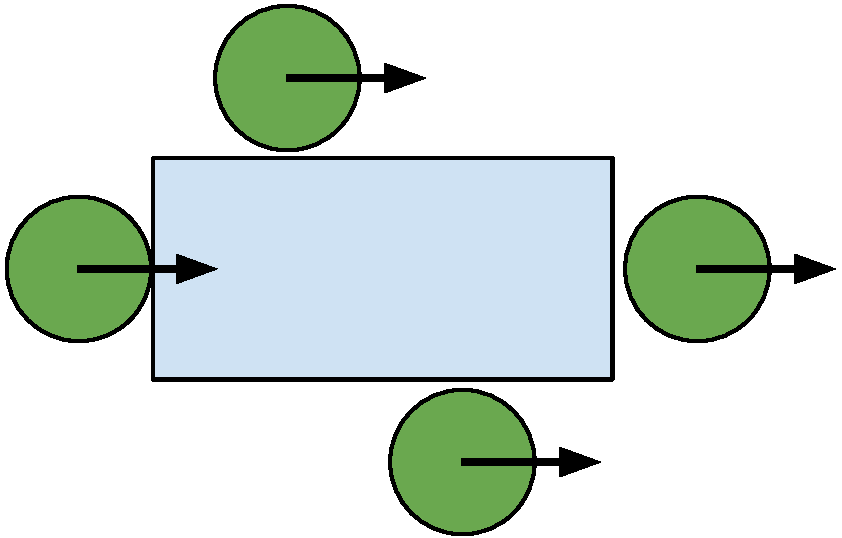
\includegraphics[width=0.9\textwidth]{img/libs/TransportTypeObjectClosure.pdf}}
    \caption{\emph{Object Closure}}
  \end{subfigure}
  \hspace{0.2cm}
  \begin{subfigure}[t]{0.45\textwidth}
    \centering
    \fbox{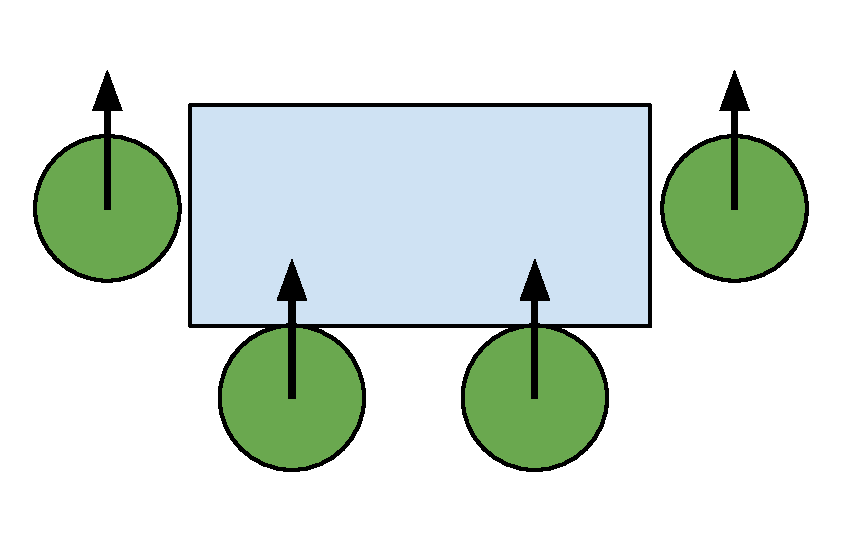
\includegraphics[width=0.9\textwidth]{img/libs/TransportTypeConditionalClosure.pdf}}
    \caption{\emph{Conditional Closure}}
  \end{subfigure}

  \caption{Conjunto das principais técnicas não-preênsil utilizadas para o transporte de objetos.}
  \label{fig:non_preensile_methods}
\end{figure}

Diversos trabalhos aplicam estas técnicas de diferentes maneiras e com modificações específicas para cada caso, além de estudar particularidades das estratégias a fim de melhorá-las.

% Trabalhos

Intuitivamente, para realização do transporte de objetos, é necessário que os agentes se aproximem do objeto e depois realizem sua manipulação. Alguns trabalhos descrevem esse processo de diferentes maneiras, propondo soluções interessantes.
%
O trabalho apresentado por \cite{Emery2001} apresenta um controlador para robôs não holonômicos, que utiliza campos vetoriais para realizar o desvio de obstáculos. Para realizar o transporte, são criados três comportamentos para os agentes: \emph{Search} -- quando o robô está procurando pelo objeto a ser transportado, \emph{Aquire} -- na qual o agente se posiciona em um local específico de acordo com a posição do objeto e do destino do mesmo, e \emph{Deliver} -- quando o agente empurra o objeto levando-o para sua pose final. As tarefas executadas são ditas como de baixa cooperação, ou seja, cada agente executa uma tarefa sozinho com fim de contribuir para objetivo final de transporte.
%
Técnicas similares são demonstradas em \cite{Song2002, Wang2002, Pereira2004, Fink2008}, nas quais ilustram um controle descentralizado, baseado em campos potenciais artificiais para navegação e desvio de obstáculos, sempre buscando utilizar os agentes para se aproximar (\emph{approach}) e circundar (\emph{surround}) o objeto em questão principalmente pelo uso de \gl{objc}, depois são aplicadas forças que atraem os agentes para a configuração final e enfim transportam (\emph{transport}) o item.

A fim de melhorar a formação e disposição na qual os agentes devem permanecer durante o transporte, \cite{Magariyama2014} apresenta a técnica chamada \emph{Feasible Dynamic Caging Zone}, na qual possibilita que agentes durante o transporte por \gl{objc} possam desviar de obstáculos ou mover o objeto para evitar uma colisão em ambientes dinâmicos, aprimorando a tarefa de forma geral.

Com uma modificação dos modelos \gl{condc} e \gl{objc}, \cite{Eoh2011} apresenta um sistema intitulado \emph{pusher-puller formation} onde dois tipos de agentes, um capaz de empurrar e outra de puxar o objeto a ser transportado, trabalham em conjunto. São definidas três diferentes técnicas para realização da tarefa:
(i) \emph{straight line} -- os agentes são posicionados atrás ou em frente ao objeto, formando uma linha reta, empurrando ou puxando o objeto respectivamente,
(ii) \emph{symmetrical formation} -- similar ao modelo anterior, porém os agentes sempre estão juntos do objeto, aplicando forças diretamente no mesmo, e
(iii) \emph{pusher-puller} -- que é o meio termo entre as estratégias anteriores, um dos agentes empurra o objeto enquanto o outro robô puxa-o. Tais modelos são exemplificados na Figura \ref{fig:eoh}.

\begin{figure}[htpb]
  \centering
  \setlength{\fboxsep}{0pt}
  \begin{subfigure}[t]{0.3\textwidth}
    \centering
    \fbox{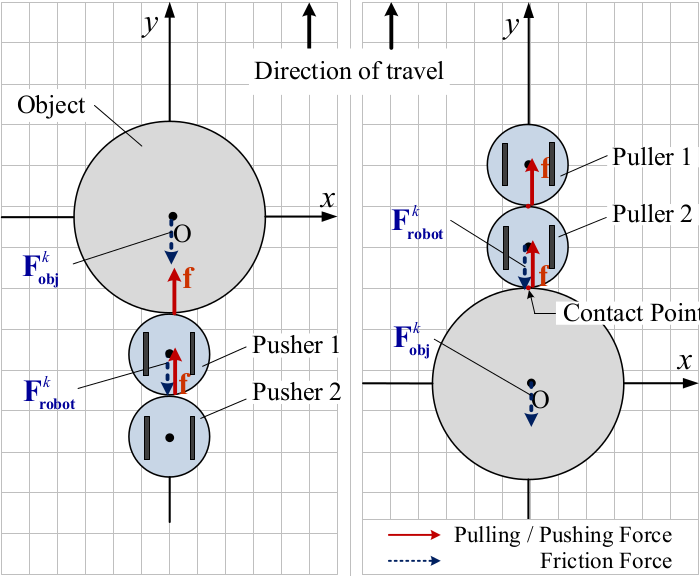
\includegraphics[width=\textwidth]{img/libs/eoh_line.png}}
    \caption{\emph{straight line}}
  \end{subfigure}
  \hspace{0.1cm}
  \begin{subfigure}[t]{0.3\textwidth}
    \centering
    \fbox{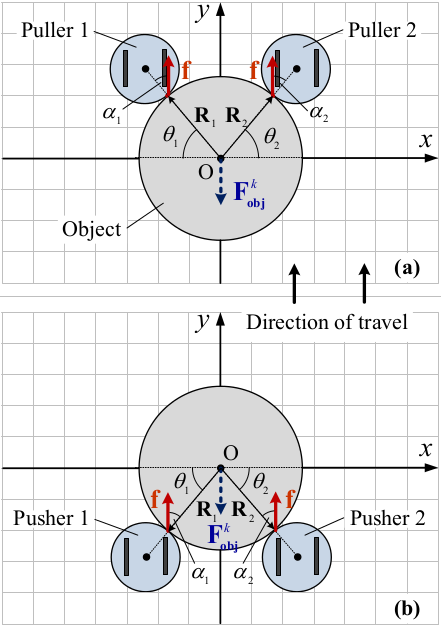
\includegraphics[width=\textwidth]{img/libs/eoh_sym.png}}
    \caption{\emph{symmetrical formation}}
  \end{subfigure}
  \hspace{0.1cm}
  \begin{subfigure}[t]{0.3\textwidth}
    \centering
    \fbox{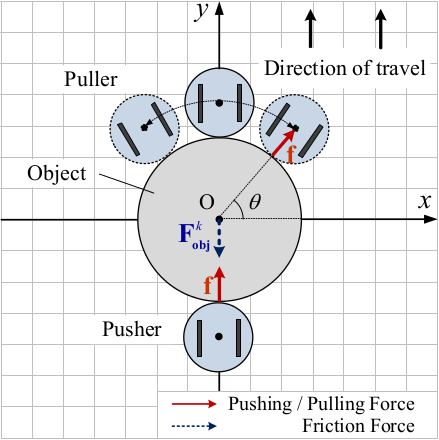
\includegraphics[width=\textwidth]{img/libs/eoh_pp.png}}
    \caption{\emph{pusher-puller}}
  \end{subfigure}

  \caption[Modelos de disposição de agentes para o transporte de objetos]{Modelos de disposição de agentes para o transporte de objetos apresentados por \cite{Eoh2011}.}
  \label{fig:eoh}
\end{figure}

O trabalho de \cite{Neumann2014} também realiza um estudo sobre a formação e posicionamento dos agentes apresentando a técnica \emph{cluster space control}, que descreve uma metodologia de modo a controlar a posição relativa entre robôs e objeto. Além disso, trata os agentes de transporte como atuadores que influenciam a movimentação do objeto, e estuda como a força aplicada sobre o mesmo determina sua trajetória e seu comportamento, salientando que comumente, trabalhos focam somente no estudo cinemático do transporte.
%
Em consenso a este trabalho, \cite{Behrens2010} discute um modelo matemático que descreve o controle da magnitude e direção da força aplicada por um agente no objeto, resultando em seu transporte.

Outro método que estuda a influência do comportamento do agente perante o objeto é demonstrado por \cite{Mericli2013}, que faz uso de algoritmos de aprendizado de máquina para criar um planejador capaz de prever a movimentação de objetos munidos de baixo atrito com o ambiente, ou seja, que uma vez empurrados, deslizam por um período de tempo.
A técnica envolve o treinamento do sistema com várias experiências de transporte, variando intensidade e tempo de duração da ação de \emph{PUSH}.
Baseado neste conhecimento, monta uma sequência de ações-reações esperadas para os objetos afim de transportá-los.
O sistema é capaz de desviar de obstáculos e recalcular o plano se as reações encontradas não condizem com o plano previamente traçado.

\cite{Gerkey2002} demonstra um modelo onde existem dois tipos de agentes, o chamado \emph{pusher}, que são capazes empurrar o objeto, enquanto o agente do tipo \emph{watcher} observa e coordena durante o desempenho do transporte. Este é um exemplo do paradigma de coordenação \emph{leader-follower} no qual o líder não faz parte diretamente da realização da missão, e faz uso do sistema de alocação de tarefas MURDOC (\cite{Gerkey2001}).

No trabalho de \cite{Costa2012} é demonstrado um sistema para transporte cooperativo no qual alguns agentes da equipe utilizam técnicas \gl{condc}. A estratégia apresentada é capaz de estimar características dos objetos (tamanho e peso) a serem transportados por meio do uso de matrizes de ocupação, além de utilizar de métodos bio-inspirados e baseados em leilão para recrutamento e alocação de tarefas dentre os robôs da equipe.

Também guiado por comportamentos encontrados na natureza, \cite{Maghsoud2014} demonstra sua técnica de transporte de objetos embasado no sistema de imunidade humana, nomeada de \emph{artificial immune system (AIS)}. Neste esquema, um time de agentes heterogêneos, possuindo diferentes capacidades de transporte, são utilizados para mover objetos com características distintas em um ambiente dinâmico. O processo de alocação dos objetos ocorre criando uma correspondência entre as capacidades do agentes e as necessidades impostas pelos itens. Tais itens são adicionados de forma arbitrária no sistema, o que o torna um exemplo de alocação \emph{online} de tarefas.

No trabalho de \cite{Ghosh2012}, o transporte de objetos é resolvido através da solução do problema denominado \emph{Multi-objective Particle Swarm Optimization}, que consiste em um algoritmo de otimização baseado no melhoramento iterativo de um conjunto de soluções guiado por uma heurística construída com base no problema a ser resolvido. O sistema apresentado busca minimizar as dimensões de tempo e energia utilizadas durante o processo, que são essencialmente dimensões conflitantes, uma vez que com maior gasto energético, ganha-se tempo, e o oposto também é válido.

Ao considerar a unidade básica do transporte por ações \emph{PUSH}, \cite{Parra-Gonzalez2008} apresenta um estudo sobre os pontos de contato entre os agentes e os objetos necessários para realização do transporte. Esta pesquisa foi aprimorada e estendida sendo apresentada por \cite{Parra-Gonzalez2011}, que descreve a utilização do algoritmo de planejamento \emph{Wavefront} (\cite{LaValle2006}) para discretizar o ambiente de trabalho e criar planos de movimentação os objetos, planos estes criados com base em três diferentes heurísticas (Figura \ref{fig:parra_object}), com diferentes objetivos: (i) busca diminuir a quantidade de mudanças de direção do objeto durante o transporte, (ii) valoriza certas orientações/rotações do objeto, pois em determinadas poses, a manipulação pelos agentes é facilitada e (iii) baseia-se em grafos, permitindo a avaliação de mais de um plano simultaneamente, onde os nós do grafo representam uma mudança na direção do transporte, e o melhor plano é aquele com a menor quantidade de nós.
Em \cite{Parra-Gonzalez2012}, os autores demonstram a utilização de planos previamente criados para os objetos, sendo explorados para o planejamento de caminhos dos agentes sempre procurando diminuir a quantidade de manobras realizadas.

% subsection manipula_o_n_o_pre_nsil (end)

\begin{figure}[h]
  \centering
  \setlength{\fboxsep}{0pt}
  \fbox{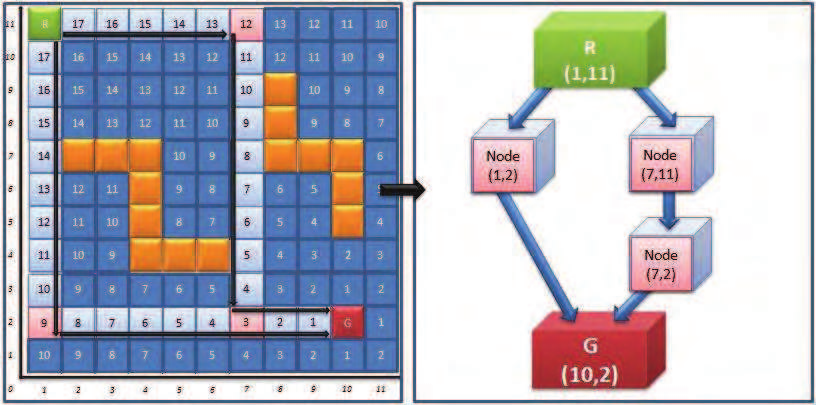
\includegraphics[width=0.7\textwidth]{img/libs/object_path_planner.png}}
  \caption[Planos de movimentação de um objeto a ser transportado]{Planos de movimentação de um objeto a ser transportado apresentados no trabalho de \cite{Parra-Gonzalez2011}. Os autores apresentam os resultados de três heurísticas distintas para o planejamento.}
  \label{fig:parra_object}
\end{figure}

\subsection{Manipulação Preênsil} % (fold)
\label{sub:manipula_o_pre_nsil}

Neste tipo de manuseio, os agentes fazem uso de manipuladores como garras ou braços robóticos para auxilar na movimentação dos objetos. Desta maneira, o item sendo transportado é preso, segurado e/ou erguido pelo agente, sendo conhecido como método \emph{GRASP}.

Antes de tornar a manipulação de objetos uma tarefa para agente móveis, alguns estudos foram realizados com manipuladores de base fixa. No trabalho de \cite{Montemayor2005}, é considerado um método para controle da movimentação e da quantidade de força exercida sobre um objeto durante o transporte. O sistema apresentado contempla uma coordenação descentralizada entre os agentes, feita mediante somente a leitura dos sensores presentes no manipulador. Este trabalho é uma extensão do trabalho de \cite{Wen1992}, que fora inicialmente concebido de forma centralizada. Outro exemplo é o apresentado por \cite{Nagai2011}, que demonstra como realizar o transporte de objetos utilizando um grua com 3 graus de liberdade realizando um planejamento de caminhos \emph{online} baseado em um mapa do ambiente, porém faz uso de sensores ultrassônicos para detectar mudanças no cenário durante o transporte.

Uma estratégia para deslocar o objeto em uma determinada direção é exposta por \cite{Ahmadabadi2001}, que cria o conceito de \emph{constrain-move}, na qual alguns agentes seguram e impedem a movimentação do objeto em certas direções, enquanto outros agentes o empurram para o destino. Esta mesma estratégia é utilizada para rotacionar o objeto, porém todos os robôs cooperam movendo o item. Ambas ações são realizadas de forma descentralizada, onde os agentes percebem o estado do objeto usando seus sensores.

Técnicas de planejamento baseadas em campos potenciais são largamente utilizadas para o transporte. \cite{Tanner2003} apresenta um método de controle centralizado que utiliza os chamados campos potenciais artificiais dipolares para criar um plano de movimentação para agentes não holonômicos possuindo manipuladores articulados, garantindo o desvio de obstáculos.
Outro caso retratado por \cite{Wada2013} utiliza robôs holonômicos e ominidirecionais, baseados em um sistema de rodas \emph{caster} ativas, os quais são capazes de erguer o objeto e transportá-lo através de portas e corredores.

Similar aos casos no qual o sistema de transporte faz uso de ações \emph{PUSH}, alguns trabalhos com \emph{GRASP} utilizam métodos de coordenação \emph{leader-follower}, como o exposto por \cite{Machado2013}, em que dois agentes são capazes de desviar de obstáculos tanto estáticos quanto dinâmicos levando um objeto longo. O robô líder transporta o item, direcionando-o para sua pose final, enquanto o dito robô \emph{helper} deve alinhar o corpo do objeto para que não colida. \cite{Sugar2002} faz algo similar, porém o objeto transportado pode ser flexível, e possui uma equipe com mais agentes. A manipulação do item ocorre com o envio da trajetória seguida pelo líder, e os demais devem segui-la, mantendo uma formação em relação ao objeto. É interessante salientar que no caso apresentado, o líder não é fixo, e pode ser realocado durante o trajeto.

O problema de transporte de múltiplos objetos também é tratado por \cite{Inoue2008, Inoue2011}, onde os robôs podem ser classificados em dois tipos: (i) única função (\emph{single-function}) -- capazes de transportar somente um objeto por vez, e (ii) multi função (\emph{multi-function}) -- aqueles que conseguem transportar mais de um objeto. Este trabalho estuda como ordenar e planejar uma sequência de transportes utilizando estes recursos.

Outra estratégia apresentada por alguns trabalhos para manipuladores móveis terrestres, é a exercitação do planejamento e controle mediante o uso de dois tipos de comando, um global e outro local. Essencialmente o planejador global deve ser capaz de criar um plano de execução do transporte considerando as limitações que o ambiente impõe, bem como as capacidades de manipulação dos agentes. O controlador local toma como base a sequência de ações a serem realizadas e monitora o desempenho dos agentes durante a tarefa, tomando as devidas decisões se algo não ocorrer como esperado, seja requisitando o replanejamento ou cancelando o transporte (\cite{Yamashita2003, Hekmatfar2014}).

No trabalho de \cite{Adorno2011} é apresentado um modelo de controle para dois braços robóticos, estendendo o trabalho apresentado em \cite{Adorno2010}, agora considerando o movimento do corpo inteiro do agente para realização da manipulação de itens com ambos manipuladores. Neste caso foi apresentado o controle cinemático de um robô com uma base móvel não holonômica, possuindo um torso e dois braços.

Um passo natural para o transporte cooperativo é a utilização de veículos aéreos para realização deste tipo de tarefa. Esta evolução garante diversas vantagens, como a extensão do ambiente de trabalho, que normalmente se limitava à movimentação em um plano (2D), e agora pode ser exercido em três dimensões. Porém também implica no aumento da complexidade do planejamento e execução da missão, onde os agentes não estão fixos, sofrendo mais facilmente de perturbações do ambiente, além de possuírem limitada capacidade de transporte, no que se relaciona ao peso e forma do objeto a ser manipulado.

Quando os agentes não são capazes de segurar o objeto através de uma garra, cabos podem ser utilizados para que o item possa ser erguido, porém esta tática acrescenta dificuldades para o controle da carga. Este problema é estudado por \cite{Michael2011} que discute um controlador para um conjunto de três agentes capaz de mensurar o equilíbrio estático do objeto, e assim descrever os comandos de movimentação dos robôs para atingir uma posição específica do objeto. Similarmente, \cite{Jiang2013} apresenta um algoritmo analítico que faz uso da técnica de eliminação dialítica (\emph{dialytic elimination}), a fim de gerar um conjunto de soluções finitas para o sistema de cinemática inversa para posicionamento do grupo (agentes e objeto). É criado o chamado \emph{tension workspace}, que limita a busca por soluções e faz o processo convergir.

Uma aplicação bastante interessante quando são utilizados agentes ágeis, como são os robôs aéreos, seja no formato de \emph{quadrotors} ou helicópteros, é o transporte e entrega de pequenos objetos, como pacotes de remédios, comunicadores, sensores e afins, em casos de missões de busca e resgate. Casos como este podem ajudar vítimas de uma catástrofe a receber ajuda de forma mais rápida quando comparados a times usuais de humanos. O trabalho de \cite{Bernard2011} demonstra este cenário, e utiliza \emph{drones} para entregar de forma precisa vários itens deste tipo, \cite{Maza2010} coordenam uma equipe de robôs para entregar em conjunto uma carga em um local previamente especificado.

Com a adição de um manipulador articulado ao robô aéreo, este conjunto pode ser tratado de duas maneiras, uma que considera as partes como separadas, e devem ser controladas independentemente, outra que julga o sistema como único, ou seja, o controle da pose do \emph{end-effector} do manipulador deve ponderar não somente as articulações do braço, mas também a liberdade garantida por um agente que se move em um espaço 3D.
Um modelo matemático pode ser derivado do sistema completo, o que proporciona o controle direto da posição onde a ação de \emph{GRASP} deve ser realizado. Este modelo pode ser aplicada em um ambiente dinâmico e considerar por exemplo erros mecânicos do aparato (\cite{Orsag2013, Kim2013}).
Seguindo um modelo similar, \cite{Arleo2013} discute um controlador hierárquico que planeja a cinemática inversa de todo o composto e o monitora durante o transporte.

No trabalho de \cite{Baizid2014} são demonstradas duas técnicas para o transporte de objetos usando \emph{drones}, ambas baseadas no método \emph{Null-Space-based Behavioral (NSB)}, que permite várias tarefas serem executadas de forma concorrente.
No cenário apresentado, dois quadrotores transportam uma barra, desviando dos obstáculos do ambiente. O primeiro método apresentado, maneja todo o conjunto para evitar colisões, já no segundo, somente o agente mais próximo ao obstáculo tem sua trajetória afetada.

Na maioria dos trabalhos, durante a etapa de captura, na qual o robô aéreo segura o objeto, ambos encontram-se em uma posição estática, ou seja, pousados sobre o solo, facilitando o manejo. Porém, existem casos onde isso não é possível, e o robô deve pegar o objeto sem pousar.
Este é o problema descrito por \cite{Pounds2011}, que cria um controlador \emph{PID} capaz de manter o agente em \emph{hovering}\footnote{permanecer parado no ar}, enquanto um objeto é pego, e posteriormente o estabiliza para transporte (Figura \ref{fig:pounds_object}).
O caso demonstrado por \cite{Thomas2014} é uma evolução deste cenário, no qual o robô aéreo não somente permanece no ar, mas também em movimento. O trabalho apresenta um manipulador inspirado nas ações de captura e transporte realizada por falcões, que é capaz de planejar a trajetória do \emph{end-effector} e manter o deslocamento do agente durante o processo de \emph{GRASP}.

\begin{figure}[h]
  \centering
  \setlength{\fboxsep}{0pt}
  \fbox{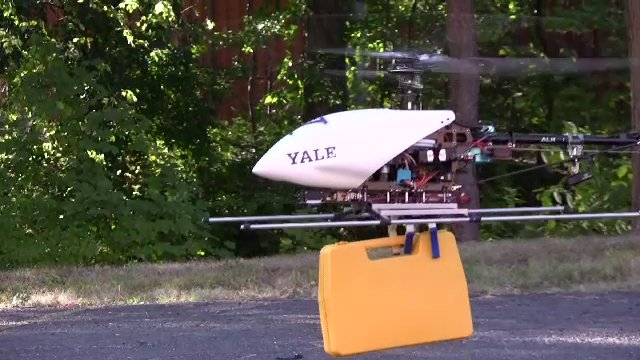
\includegraphics[width=0.7\textwidth]{img/libs/quad_transport.png}}
  \caption[Transporte realizado por um quadrotor que utiliza uma garra para segurar o objeto]{Transporte realizado por um quadrotor que utiliza uma garra para segurar o objeto demonstrado por \cite{Pounds2011}.}
  \label{fig:pounds_object}
\end{figure}

Outra aplicação interessante, uma vez que agentes aéreos são capazes de transportar objeto, é a criação de estruturas de forma autônoma.
Uma maneira demonstrada em alguns trabalhos é a utilização de elementos pré-fabricados que possam ser conectados facilmente, como é o caso do chamado \emph{Special Cubic Structures (SCS)}, peças como barras e juntas, possuem imãs e são facilmente encaixadas (\cite{Lindsey2011, Lindsey2012}).
Partindo do mesmo conceito, os trabalhos de \cite{BarrosdosSantos2013, BarrosdosSantos2014} descrevem um \emph{framework} que cria um esquema adaptativo a partir de algoritmos de aprendizado de máquina (treinamento por reforço). Este \emph{framework} criar planos de alto nível em um simulador e posteriormente acompanha a execução da construção em robôs reais.

Outro exemplo de construção usando agente autônomos é o nomeado \emph{Aerial Robotic Construction (ARC)}, o qual define um estudo sobre a mudança nos paradigmas de design e fabricação de itens.
Na pesquisa são expostos algumas vantagens deste sistema:
(i) a construção das estruturas não necessita de armações de apoio para ser realizado,
(ii) o modelo digital pode ser complexo, e os agentes são guiados explicitamente por este, e
(iii) o sistema é escalável no sentido de não estar preso ao ambiente, além de poder escalar um grande equipe capaz de atuar simultaneamente durante o processo (\cite{Willmann2012, Augugliaro2014}).

% subsection manipula_o_pre_nsil (end)
% section t_cnicas_de_manipula_o_de_objetos (end)

\section{Alocação de Tarefas e Coordenação} % (fold)
\label{sec:t_cnicas_de_aloca_o_de_tarefas}

Ao considerar que diversas atividades, como é o caso do transporte cooperativo, possuem um conjunto de subtarefas que devem ser realizadas para completar a tarefa principal, a etapa de alocação de tarefas compreende o estudo e organização deste conjunto, de modo a selecionar os melhores agentes para realização de cada subtarefa específica.
Após esta etapa, surge a necessidade de coordenar os agentes para que realizem suas atividades de forma sincronizada e cooperativa.

Os trabalhos citados a seguir demonstram e estudam algumas técnicas empregadas principalmente em ambas estas etapas, discutindo métodos distintos, com suas próprias vantagens e desvantagens.

Neste sentido, \cite{Shiroma2009} apresenta em seu trabalho o \textit{framework} CoMutaR (\emph{Coalition formation based on Multitasking Robots}), que descreve um método para alocação e coordenação de agentes multi-tarefas para realização de diversas tarefas.
É baseado na suposição de que uma dada tarefa pode ser dividida em partes atômicas, denominadas ações; cada ação possui restrições e recursos necessários para ser ativada. Uma coleção de ações ativáveis resulta na realização da tarefa.

Outra proposta é apresentada por \cite{Carvalho2013}, que pretende distribuir uma equipe de agentes para exploração de uma extensa região aplicando técnicas de coloração de grafos para selecionar qual robô deve ir para qual região.
\cite{Kulatunga2006} apresenta uma técnica que busca planejar caminhos e alocar tarefas simultaneamente entre agente aéreos usando como base comportamentos inspirados em formigas.

É apresentado por \cite{Tiganas2013} uma técnica na qual agentes devem coletar e transportar amostras de uma região para outra, os mesmo são capazes de identificar e modificar seu comportamento mediante a necessidade do sistema, coordenando-se para coletar mais em uma determinada fonte ou entrar em modo de espera, por exemplo.
Também apresentando uma estratégia para ambiente dinâmicos, \cite{Wang2009} descreve a utilização de grafos para a coordenação e mudança de classes de agentes dentro do simulador de futebol \emph{RoboCup Soccer}.

Estas técnicas, além de suas variações e expansões são aplicadas em diferentes contextos, como no trabalho de \cite{Sujit2013}, que apresenta uma avaliação empírica de algumas estratégias de coordenação entre robôs heterogêneos com a missão de explorar uma determinada área a fim de coletar dados sobre a água para casos como o rastreamento de óleo, medida de gradientes de temperatura ou proliferação de algas nocivas, apresentando três táticas de coordenação:
(i) periódica -- que ocorre em intervalos pré-determinados de tempo,
(ii) distância -- que busca percorrer uma área com um plano de menor tamanho e
(iii) probabilística -- onde a coordenação ocorre em tempos adaptativos.
%
Também buscando a cooperação entre agentes de diferentes tipos, \cite{Grocholsky2006} demonstra uma técnica de localização de alvos em uma região, usando um princípio descentralizado de controle implementando comportamentos diferentes para tipos de agentes.

Demonstrando como aplicar a técnica \emph{AlphaBeta}, \cite{Goldsmith1998} descreve seu uso na exploração de ambientes, onde não é possível uma supervisão direta e o sistema deve ser robusto o suficiente para funcionar sem intervenção.
O grande diferencial desta técnica de coordenação está na diferença complementar de comportamentos entre as duas equipes, enquanto uma explora o ambiente, motivados por achar novas regiões não exploradas, a outra equipe segue os caminhos já gerados, economiza energia, gerando uma melhor leitura do ambiente.
Neste mesmo sentido, \cite{Tanner2007} também apresenta uma coordenação \textit{AlphaBeta}, mas agora para robôs terrestres e aéreos, para a tarefa de monitoramento de uma área a fim de detectar e rastrear intrusos.

Especificamente em relação ao controle e coordenação de uma equipe de agentes, é possível listar uma série de modelos que compreendem esta etapa, com diferentes aplicações e características.

Na técnica comportamental (\emph{Behavior Based}), a organização dos agente no sistema é realizada através da associação de comportamentos aos mesmos, definidos como um conjunto de ações que são mapeadas diretamente dos sensores para os atuadores do robô. Estes comportamentos podem ser dispostos como uma máquina de estados finitos, promovendo uma mudança de atitude dos robôs mediante necessidade.
No trabalho de \cite{Brooks1986}, é explanado a criação de um comportamento mais complexo baseado na disposição hierárquica de procedimentos mais simples. Deste modo, a ação executada será aquela resultante da junção de todas as saídas depois de passar pelos níveis do comportamento.
Uma vantagem notável é a possibilidade da atuação de diversas condutas concorrentemente. Um aditivo a tal possibilidade seria a priorização de certos comportamentos, como por exemplo, o desvio de obstáculos. Em contraste a esta vantagem, a adição de mais níveis de controle aumenta a complexidade da tomada de decisão, que pode tornar o sistema intratável.

Outros formatos de coordenação são aqueles biologicamente inspirados (\emph{Biologically Inspired}), na qual o controle dos agentes é baseada em traços biológicos, na tentativa de implementar mecanismos que foram desenvolvidos e testados na natureza no âmbito de sistema robóticos. Observando animais de diversos tipos, como insetos, é possível extrair características comportamentais para ações como exploração ou navegação (\cite{Kube2000}).

Uma das técnicas bastante utilizada, como visto em alguns trabalhos de transporte cooperativo, é a coordenação \emph{AlphaBeta}, que pode ser aplicada como uma camada superior às demais técnicas de coordenação, pois, apesar de influenciar diretamente no comportamento do grupo, é tratado como um aditivo, e não como um substitutivo. Este método consiste na divisão da equipe de agentes em duas sub-equipes com objetivos complementares, seja pelo caso de um time preparar o ambiente para o outro ou servir como uma equipe sensorial, por exemplo.
As duas equipes podem trabalhar simultaneamente, trocando informações pertinentes em tempo real, ou podem funcionar em modo comutado (\emph{switched}), ou seja, enquanto um atua, o outro espera pelos resultados para só então entrar em ação (\cite{Goldsmith1998}).

Existem também dois tipos de controle que geralmente são aplicados em uma camada acima dos demais citados anteriormente.
O controle centralizado é baseado na coordenação e tomada de decisão considerando um líder, que deve processar e distribuir as tarefas dentre todos os membros da equipe. Os demais componentes do sistema recebem ordem e retornam relatórios de suas ações.
Esta estratégia se destaca na velocidade em que todos os agentes da equipe tomam ciência de suas atribuições, sem necessidade de acordos ou negociações. A grande penalidade se encontra na parte comandante, que, se houver falhas, todo o sistema pode sofrer uma falha (\cite{Farinelli2004, Miyata2002}).

De forma contrária, no controle descentralizado, todos os integrantes do grupo participam das diversas etapas de que o sistema pode necessitar, como o sistema de coordenação e alocação de tarefas. A sincronização entre os agentes é feita mediante a troca de informações referentes às decisões individuais e posterior comunicação com os demais agentes.
Neste caso, uma maior tolerância a falhas é agregada ao sistema, pois, mesmo que um agente pare de funcionar, os demais agentes podem continuar a execução da tarefa. Porém, neste tipo de controle, os agentes devem entrar em consenso sobre a responsabilidade das tarefas, o que pode acarretar um acréscimo no tempo total das atividades (\cite{Farinelli2004}).

\section{Abordagem Proposta} % (fold)
\label{sec:abordagem_proposta}

Neste trabalho, será apresentada um série de técnicas que propõem metodologias para o controle e coordenação de agentes para realização do transporte e manipulação de objetos utilizando uma equipe heterogênea de robôs.

Em contraste com a maioria dos trabalhos listados, a estratégia apresentada se baseia na trajetória criada para cada objeto a ser transportado, plano este que considera os recursos disponibilizados pelos robôs dentro do sistema.
Comumente, o transporte de objetos é realizado baseado nos trajetos que os agentes devem realizar, uma vez que estes, utilizando táticas preênsil por exemplo, se deslocam e por consequência, transportam o objeto.

A etapa de mapeamento não é contemplada pela técnica, considerando que existe conhecimento dos estados e localidades de cada obstáculo, objetos e agentes dentro do ambiente de trabalho.
O mapa criado como base para a tarefa compreende o método de segmentação celular em forma de matriz para dispor e descrever estas informações espacialmente.

Baseado na pré-existência do mapa, o foco desta pesquisa se encontra principalmente em como alocar tarefas e coordenar os agentes, de modo que dimensões como a distância percorrida, energia gasta e o tempo total da atividade sejam minimizados considerando as necessidades do sistema.
Para tal, foi desenvolvida uma função de utilidade que considera tais dimensões, bem como a disparidade entre os tipos dos agentes, compreendendo um ambiente com robôs heterogêneos.

O controle e coordenação dos agentes será realizada de forma descentralizada, garantindo vantagens em tempo de planejamento, pois as atividades são separadas dentre a equipe, sendo realizadas de forma simultânea.

\section{Comparativo} % (fold)
\label{sec:comparativo}

A Tabela~\ref{table:related_works} apresenta um demonstrativo dos trabalhos relacionados à área de transporte cooperativo, salientando as áreas em que mais tiveram atuação dentro da pesquisa, além de elencar os campos que o presente trabalho possui contribuições.

\begin{sidewaystable}

% \begin{table}[]
\centering
\caption{Tabela demonstrativa das pesquisas no campo do transporte de objetos elencando as principais áreas de atuação.}
\label{table:related_works}
\begin{tabular}{l|c|c|l|c|c|c|}
\cline{2-7}
                                                & \multicolumn{2}{c|}{Foco de Transporte}       & \multicolumn{2}{c|}{Tipo de Transporte}                & \multicolumn{2}{c|}{Coordenação}              \\ \cline{2-7}
                                                & Objeto                & Agentes               & \multicolumn{1}{c|}{Preênsil} & Não-Preênsil           & Centralizada          & Descentralizada       \\ \hline
\multicolumn{1}{|l|}{\cite{Pereira2004}}        &                       & x                     & \multicolumn{1}{c|}{}         & x                      &                       & x                     \\ \hline
\multicolumn{1}{|l|}{\cite{Fink2008}}           &                       & x                     & \multicolumn{1}{c|}{}         & x                      &                       & x                     \\ \hline
\multicolumn{1}{|l|}{\cite{Behrens2010}}        & \multicolumn{1}{l|}{} & x                     & \multicolumn{1}{c|}{x}        & \multicolumn{1}{l|}{}  & x                     & \multicolumn{1}{l|}{} \\ \hline
\multicolumn{1}{|l|}{\cite{Eoh2011}}            & x                     & x                     &                               & x                      & x                     & \multicolumn{1}{l|}{} \\ \hline
\multicolumn{1}{|l|}{\cite{Inoue2011}}          & x                     & \multicolumn{1}{l|}{} &                               & x                      & \multicolumn{1}{l|}{} & x                     \\ \hline
\multicolumn{1}{|l|}{\cite{Nagai2011}}          & x                     & \multicolumn{1}{l|}{} &                               & x                      & x                     & \multicolumn{1}{l|}{} \\ \hline
\multicolumn{1}{|l|}{\cite{Costa2012}}          & x                     & x                     &                               & x                      & \multicolumn{1}{l|}{} & x                     \\ \hline
\multicolumn{1}{|l|}{\cite{Parra-Gonzalez2012}} & \multicolumn{1}{l|}{} & x                     & \multicolumn{1}{c|}{x}        & \multicolumn{1}{l|}{}  & \multicolumn{1}{l|}{} & x                     \\ \hline
\multicolumn{1}{|l|}{\cite{Arleo2013}}          & x                     & \multicolumn{1}{l|}{} &                               & x                      & x                     & \multicolumn{1}{l|}{} \\ \hline
\multicolumn{1}{|l|}{\cite{Jiang2013}}          & x                     & \multicolumn{1}{l|}{} & \multicolumn{1}{c|}{x}        & \multicolumn{1}{l|}{}  & x                     & \multicolumn{1}{l|}{} \\ \hline
\multicolumn{1}{|l|}{\cite{Machado2013}}        & x                     & \multicolumn{1}{l|}{} &                               & x                      & x                     & \multicolumn{1}{l|}{} \\ \hline
\multicolumn{1}{|l|}{\cite{Mericli2013}}        & \multicolumn{1}{l|}{} & x                     & \multicolumn{1}{c|}{x}        & \multicolumn{1}{l|}{}  & x                     & \multicolumn{1}{l|}{} \\ \hline
\multicolumn{1}{|l|}{\cite{Orsag2013}}          & x                     & \multicolumn{1}{l|}{} &                               & x                      & x                     & \multicolumn{1}{l|}{} \\ \hline
\multicolumn{1}{|l|}{\cite{Kim2013}}            & x                     & \multicolumn{1}{l|}{} &                               & x                      & x                     & \multicolumn{1}{l|}{} \\ \hline
\multicolumn{1}{|l|}{\cite{Wada2013}}           & x                     & \multicolumn{1}{l|}{} & \multicolumn{1}{c|}{x}        &                        & \multicolumn{1}{l|}{} & x                     \\ \hline
\multicolumn{1}{|l|}{\cite{Hekmatfar2014}}      & x                     & \multicolumn{1}{l|}{} & \multicolumn{1}{c|}{x}        & \multicolumn{1}{l|}{}  & x                     & \multicolumn{1}{l|}{} \\ \hline
\multicolumn{1}{|l|}{\cite{Magariyama2014}}     & \multicolumn{1}{l|}{} & x                     &                               & x                      & \multicolumn{1}{l|}{} & x                     \\ \hline
\multicolumn{1}{|l|}{\cite{Maghsoud2014}}       & x                     & x                     &                               & x                      & \multicolumn{1}{l|}{} & x                     \\ \hline
\multicolumn{1}{|l|}{\cite{Neumann2014}}        & \multicolumn{1}{l|}{} & x                     &                               & x                      & \multicolumn{1}{l|}{} & x                     \\ \hline
\multicolumn{1}{|l|}{Este Trabalho}             & x                     & x                     & \multicolumn{1}{c|}{x}        & x                      & \multicolumn{1}{l|}{} & x                     \\ \hline
\end{tabular}
% \end{table}

\end{sidewaystable}

% chapter trabalhos_relacionados (end)
